\documentclass[journal]{IEEEtran}

\ifCLASSINFOpdf
\else
\fi

% correct bad hyphenation here
\hyphenation{op-tical net-works semi-conduc-tor}
\usepackage[british]{babel}
\usepackage[hidelinks, unicode]{hyperref}
\usepackage[utf8]{inputenc}
\usepackage[T1]{fontenc}
\usepackage{amsmath}
\usepackage{bm}
\usepackage{amsfonts}
\usepackage{float}

\usepackage{graphicx}
\graphicspath{ {./images/} }

\usepackage{cleveref}

\begin{document}

\title{\vspace{-0.5em}DarkrAI: a Pareto \bm{$\varepsilon$}-greedy policy\\[0.1em]\huge \textit{Improving Pokémon AI Training With NSGA-II}}
\author{\href{https://github.com/Simone-Alghisi}{Simone Alghisi}, \href{https://github.com/samuelebortolotti}{Samuele Bortolotti}, \href{https://github.com/massimo-rizzoli}{Massimo Rizzoli}, \href{https://github.com/erich-r}{Erich Robbi}\\Department of Information Engineering and Computer Science\\University of Trento, Italy\\

\normalsize\{\href{mailto:simone.alghisi-1@studenti.unitn.it}{\texttt{simone.alghisi-1}},  \href{mailto:samuele.bortolotti@studenti.unitn.it}{\texttt{samuele.bortolotti}}, \href{mailto:massimo.rizzoli@studenti.unitn.it}{\texttt{massimo.rizzoli}},  \href{mailto:erich.robbi@studenti.unitn.it}{\texttt{erich.robbi}}\} \texttt{@studenti.unitn.it}\vspace{-1em}}%

% make the title area
\maketitle

% As a general rule, do not put math, special symbols or citations
% in the abstract or keywords.
\begin{abstract}
Nowadays, Reinforcement Learning is one of the most popular strategies to train agents able to play different games. In particular, Deep-Q Learning aims to achieve this by maximising the expected cumulative reward for future states (i.e. utility). However, while such strategy is problem agnostic, it requires an enormous amount of time to converge to a stable result. In Pokémon games, Double Battles have an extremely high complexity: in particular, there are at most $306$ different turn outcomes for each player. In this scenario, removing especially useless moves to speed up the training is fundamental. In this paper, we discuss the effectiveness of employing \emph{NSGA-II}, a Genetic Algorithm, for training a Pokémon agent with a controlled search by solving a multi-objective optimisation problem.
\end{abstract}

\begin{IEEEkeywords}
Reinforcement Learning, NSGA-II, Multi-objective Optimisation, Genetic Algorithms
\end{IEEEkeywords}

\IEEEpeerreviewmaketitle

\section{Introduction}
\label{sec:intro}
\IEEEPARstart{P}{okémon} is a popular turn-based game where two players must choose a monster move and a target each turn with the aim of knocking out all the opponent's Pokémons. The game is far from being trivial and has many different possible strategies, leading to a very high-dimensional search space. Moreover, each of the player's Pokémon has unique statistics\footnote{\url{https://bulbapedia.bulbagarden.net/wiki/Stat\#List_of_stats}} such as Speed, HP (Health Points), Attack, and Defence. The fact that the opponent Pokémons also have their own unknown parameters makes the game even more convoluted. In particular, there are $10^{354}$ different ways a Pokémon battle can start, and each turn has at most $306$ different outcomes (and only for a single player). The game's complexity turns out to be a problem for the development of a Pokémon AI, as high complexity implies a very large number of possible outcomes to choose from. Since the analysis of all possibilities is not feasible, it is imperative to implement a strategy to efficiently find an ideal move. At the beginning of a \emph{Reinforcement Learning (RL)} training procedure, an agent does not know which action is the most effective in order to win the battle. The purpose of this study is to give the Pokémon AI agent a set of potentially useful moves to warm up the training process and have a faster training convergence. Since each move has a different effect on the game and it is driven by the dynamics of the combat, the term "useful move" is ambiguous and there is no one-size-fits-all approach. Genetic Algorithms, in particular \emph{NSGA-II}, allow to produce \emph{Pareto-equivalent} solutions of a multi-objective optimisation problem, which is suitable in order to find the best move a Pokémon can perform.

\section{Approach}
\label{sec:approach}
In this study, we have applied bio-inspired methods to enhance RL performances and speed up the learning process. Firstly, we have devised a \texttt{node} server in order to compute the damage each move can deal. Secondly, we have set up NSGA-II so as to solve an optimisation problem and return the Pareto optimal moves the Pokémons can make in the current turn. Thirdly, we have designed an \emph{Artificial Neural Network (ANN)} whose weights are learned through RL. Finally, we have evaluated our solution in terms of reward and winrate.

\subsection{Damage calculator}
The most trivial way to take a good move is to select the one which inflicts the highest possible damage. However, such information is difficult to retrieve since it depends on several factors (e.g. weather conditions, Pokémon statistics, etc).

To compute the effects of a Pokemon move against an opponent we have set up a \texttt{node} web server infrastructure, which allows us to interface with a damage calculator \emph{Application Programming Interface (API)} server\footnote{\url{https://github.com/smogon/damage-calc}}. By doing so, we can process several requests simultaneously with little latency, since it runs locally, and acts as a glue between different libraries. In fact, our Python program can communicate with it to obtain the required information about the effectiveness of a move.

\subsection{Genetic Algorithm}
The data returned from the damage calculator is then used together with genetic algorithms to solve a multi-objective optimisation problem, by employing NSGA-II.

\subsubsection{Genetic Representation}
To find out which move is the best, we need to at least look at the current turn. Generally, in a Pokémon battle two actions are possible, i.e. performing a move or a switch. Moreover, depending on the type of battle, it may be necessary to specify the target of the move. To encode such a thing, we came up with the following genotype: each Pokémon is represented using two genes, i.e. action and target (optional) $(a, t)$. The whole genotype tells us who is going to perform what on whom. Despite being straightforward, it is mandatory to avoid illegal actions, e.g. choosing the same switching tactic for two different Pokémons.

However, in most of the cases, information regarding the opponent's Pokémons is not known. Thus, to overcome this problem we have employed the data available on \texttt{pikalytics}\footnote{\url{https://www.pikalytics.com/}}, which provides competitive analysis and team building help. Therefore, by using a web scraper, it is possible to get the most popular settings and moves for each Pokémon as determined by expert players. As a result, \emph{NSGA-II} always has a decent knowledge of the opponent's team because it considers the most likely moves under uncertainty.

\subsubsection{Mutation and Crossover}
Mutation is performed for each gene in a genotype with  probability $\mathbb{P}_m = 10\%$: both the action and the target may be mutated, meaning that it is possible to go from a move to a switch (and vice-versa). For this reason, we had to check the validity of the new action, and change it accordingly otherwise.
Instead, we used Uniform Crossover in a particular way: given that each Pokémon is represented by a valid $(a, t)$ pair, we perform crossover by selecting the whole pair from one of the parents to avoid inconsistencies. Furthermore, crossover is performed with $\mathbb{P}_c = 100\%$, and $\mathbb{P}_{bias} = 50\%$ (i.e. the bias towards a certain offspring). Moreover, we developed a custom repair algorithm that transforms an unfeasible solution into a feasible one.

\subsubsection{Search Strategy}
\label{subsec:search}
We used \emph{NSGA-II} with the aim of approximating a \emph{Pareto Front}. Our optimisation problem can be defined as follows:
\begin{equation*}
    \underline{x} = (x_1,x_2,x_3,x_4) \in \mathbb{R}^4
\end{equation*}
where $x_1$ is the damage dealt by the ally Pokémons (\texttt{MON DMG}) to the opponents, $x_2$ is the damage dealt by the opponents' Pokémons (\texttt{OPP DMG}) to the allies, $x_3$ is the health points remaining of the player's Pokémons (\texttt{MON HP}), $x_4$ is the health points remaining of the opponent's Pokémons (\texttt{OPP HP}), and $\mathbb{R}^4$ is our search space, defined as:
\begin{equation*}
    \mathbb{R}^4 = \{(x_1,x_2,x_3,x_4) : 0 \leq x_1,x_2,x_3,x_4 \leq 100\}
\end{equation*}
This leads to the following multi-objective problem:
\begin{equation*}
    \max_{\underline{x} \in \mathbb{R}^4} f(\underline{x}) = (f_1(x_1),f_2(x_2),f_3(x_3),f_4(x_4))
\end{equation*}
where $f(\underline{x})$ is our objective vector that we want to maximise. 
Hence, the Pareto optimal rounds are the ones which maximise the damage dealt by both ally and opponent teams, while jointly preserving as many health points as possible from both sides. Therefore, the move we are looking for is not only the best one for the ally team, but also the optimal one for the opponent team. This is motivated because if there exists an optimal move for the opponent, we assume that the opponent is going to perform it. The generation of the Pareto Front will rely greatly on the damage calculator server, as the latter provides the values of $\underline{x}$.

\subsubsection{Fitness Evaluation}
As introduced in \Cref{subsec:search}, our problem is made of 4 different objectives that need to be maximised. However, to make the computation as reliable as possible, we need to consider other elements that could affect the damage. For example, the turn order depends on the Pokemons' Speed and the Priority of their actions, meaning that a Pokémon may faint before acting if a certain condition is met. Thus, its damage should not be considered for the global objective. Instead, if a switch is encoded in the genotype, the damage should be done on the entering Pokémon.

For this reason, the evaluation is performed by considering run-time elements, such as the action and the Pokémon encoded in the current genotype. Thanks to this, a turn order can be estimated, and the HP of the on-field Pokémon are considered to enhance precision. Moreover, such estimates are updated at each turn upon receiving new observations.

\subsection{Reinforcement Learning}
The reinforcement learning technique we have employed is called \emph{Deep Q-Learning}, which shares the same idea of \emph{Q-Learning (QL)}, but it employs an ANN. QL is based on the Q-function, namely $Q : S \times A \rightarrow R$, which returns - given a state-action pair ($s, a \in S \times A$) - the expected discounted reward ($r \in R$) for future states. The core idea behind RL is that an agent chooses an action $a$ in the current state $s$, then performs it, and observes the outcome which will produce a new state $s'$; finally, it measures the associated reward $r$. The learning proceeds by updating the Q-function thanks to the \emph{Bellman Equations}:
\begin{equation*}
    Q(s_t, a_t) \leftarrow Q(s_t, a_t) + \alpha \Big[ r_{t + 1} + \gamma \max_{a} Q(s_{t + 1}, a) - Q(s_t, a_t)\Big]
\end{equation*}

where $\alpha$ is the learning rate, $a_t$ is the action taken by the agent at time $t$ when at state $s_t$, and $r_{t + 1}$ is the reward obtained at time $t + 1$. $\gamma$ is the discount factor, a trade-off parameter that helps the algorithm to converge, scaling down future rewards.

In this work, we have considered \emph{$\varepsilon$-greedy action selection}: with a small probability $\varepsilon$ the algorithm chooses to explore, i.e. performs a random move; otherwise, it exploits, i.e. performs the action with the highest reward.

At inference time, the agent selects the action which maximises the Q-value.

\subsubsection{Architecture}
The agent architecture is a four-layer deep \emph{Multilayer Perceptron (MLP)}, which employs \emph{ReLU} as activation function. The structure consists of one input layer whose size depends on the type of battle the network is facing (e.g. a $4 \text{ VS } 4$ battle implies a size of $244$ input neurons), two hidden layers respectively of size $256$ and $128$, and an output layer which consists of $621$ neurons, i.e. all the possible combinations of moves.

% TODO: PENSARE A UN NOME PIU DECENTE SE LO TROVIAMO ALTRIMENTI NIENTE LASCIAMO COSI
\subsubsection{State description}
Among all the possible information that can be considered, we focused on the following: the percentage of Pokémons alive, the weather, and the field condition; then, for each Pokémon we consider their type\footnote{\url{https://bulbapedia.bulbagarden.net/wiki/Type}} (e.g. fire, grass, ...), HP percentage, statistics (normalised), status\footnote{\url{https://bulbapedia.bulbagarden.net/wiki/Status_condition}} (e.g. asleep, poisoned, ...); lastly, for each Pokémon's move, we consider its id, priority, type, and damage it deals to the opponent active Pokémons. Other useful information may be considered; however, the problem becomes exponentially more difficult due to the curse of dimensionality.

\section{Experiments}
\label{sec:exp}
% TODO: con grafici e statistical analysis (le immagini le mettiamo nell'appendice, tranquilli abbiamo visto Reports di 6 pagine di cui 4 di testo e 2 appendice.
% qua descriviamo a parole immagini e figure.

% Cosa vogliamo provare, che test e analisi andremo a fare e difficulties

% TODO: parlare qua o altrove di tutti gli agenti?
 
The learning was carried out through \texttt{poke-env}\footnote{\url{https://github.com/hsahovic/poke-env}}, a Python environment for training RL Pokémon agents, which interfaces with Pokemon Showdown\footnote{\url{https://pokemonshowdown.com/}}, a Pokémon battle simulator. As it concerns the $\varepsilon$-greedy policy, we started from a probability $\mathbb{P}_r=1.0$ to perform a random action, which linearly decreases to $\mathbb{P}_r=0.1$ in the first $40\%$ of the training. Then, for the remaining $60\%$ of the training, it linearly decreases to $\mathbb{P}_r=0.01$.

To create an environment as stable as possible, all agents were trained by having them fight against \textit{MaxDamagePlayer}, i.e. a bot which always chooses the combination of moves that deals the highest amount of damage. Despite seeming deterministic, there is some level of stochasticity which cannot be controlled during training, e.g. additional effects such as freeze, critical hits, etc.
% Descrivere nel dettaglio che fanno i player e come sono stati allenati

\subsection{Player}
The first Pokémon Agent has been trained using only the RL facilities provided by \texttt{poke-env}. The idea is quite straightforward: the $\varepsilon$-greedy described above is employed for the training of the network for a certain number of epochs.

\subsection{ParetoPlayer}
ParetoPlayer embeds the Pareto search of non-dominated turns, according to \Cref{subsec:search}. To this end, we changed the policy of the previous agent to perform a random move chosen from the ones returned by \emph{NSGA-II} with $70\%$ probability, while a completely random one with $30\%$ probability. The idea is that, given that the search space is very big, we would like to positively bias our model with a controlled search, removing particularly useless moves. However, to avoid biasing the search too much, such behaviour is carried out only for the first $20\%$ of the training: after that, the $\varepsilon$-greedy policy will only suggest random moves, going back to full exploration. Finally, we set for \emph{NSGA-II} a population size of $20$ paired with $20$ generations, since we saw that it was a good trade-off between performance and quality of the results.

\section{Analysis}
\label{sec:analysis}
% statistical results and their significance
In order to assess our experiments we have employed some data analysis techniques, such as statistical tests and plots, to show whether the employment of \emph{NSGA-II} as a warm-up for RL is beneficial or not.

\subsection{Normality} 
The first test we have conducted is concerning the data normality. These tests are used to determine if a data set is well represented by a normal distribution. Moreover, this information can be useful in order to run a \emph{t-test} since it assumes that the measurements are normally distributed.

To fulfil this request, we have employed graphical methods such as \emph{quantile-quantile plot}, which is useful to compare two probability distributions by plotting their quantiles against each other, and two statistical tests such as the \emph{Shapiro-Wilk test}\footnote{\href{https://en.wikipedia.org/wiki/Shapiro\%E2\%80\%93Wilk_test}{https://en.wikipedia.org/wiki/Shapiro-Wilk\_test}} and a \emph{Kolmogorov Smirnov test}\footnote{\href{https://en.wikipedia.org/wiki/Kolmogorov\%E2\%80\%93Smirnov_test}{https://en.wikipedia.org/wiki/Kolmogorov-Smirnov\_test}}. Both statistical tests work by assuming as null hypothesis that the sample distribution is normal, while as alternative hypothesis that sample distribution is not normal. However, Shapiro test is suitable with few observations whereas Kolmogorov is capable of handling more observations.

\subsection{Statistical significance} 
To observe whether Pareto has brought an improvement with respect to classic RL, we have used \emph{box plots}, the \emph{t-test}, and the \emph{Wilcoxon rank mean test}.
Box plots are graphical method to display the data distribution grouping them through their quartiles, while the t-test and Wilcoxon test are two analytical techniques for determining if a difference between two distributions is statistically significant. The t-test assumes normal data, whereas the non-parametric Wilcoxon test can be used with both normal and non-normal data.

\subsection{Empirical Results}
The data we have considered for the analysis of ParetoPlayer and Player are the \emph{episode reward}, namely the average amount of reward the agent gets in a single game, and the \emph{winrate}, which is the percentage of battles won. To this end, we prepared three different 2 VS 2 battles to test the capability of the proposed method: one where both the network and the opponent keep the same teams across the training; one where the teams are still fixed, but there exists a single win condition; and one where the opponent team is sampled randomly from a pool. In particular, for each method, we first performed $10$ training runs with both Player and ParetoPlayer, and then a row-wise mean operation (for each episode, we take the mean of the $10$ rewards) to have two stabler curves for testing purposes.

Regarding the first set of experiments, we found a significant improvement in terms of episode reward for ParetoPlayer w.r.t. Player. As shown by the Kolmogorov-Smirnov, the reward per episode from ParetoPlayer is stochastically greater than the one from Player, meaning that $F_{pp}(x) \leq F_p(x)$ and hence $\mathbb{E}[X_{pp}] \geq \mathbb{E}[X_p] $ with a $p$-value of $p < 2.2 \cdot 10^{-16}$. This trend has been observed also from the box plots when considering $1000$ random battles performed by the agents with the highest reward. In particular, ParetoPlayer's box plot is basically flat, with the majority of points almost equal to the median, while the outliers are more concentrated either nearby or above the median value. Instead, Player's box plot shows that the distribution of the rewards has higher variance with the median slightly lower than the one of ParetoPlayer, and it accounts for more negative values. However, the Wilcoxon rank-sum test, that given $X$ and $Y$ randomly sampled from two populations measures whether the likelihood of $X$ being bigger than $Y$ is equal to the probability of $Y$ being greater than $X$, shows that in some cases the episode reward distribution is shifted to the right, thus greater than the one obtained from the Player (i.e. $p$-value is $2.886 \cdot 10^{-12}$), and in some other they are almost equivalent (i.e. $p$-value of $0.94$). Regarding the win rate, the test has shown that the data distribution of the ParetoPlayer is shifted to the right than the one obtained from Player (i.e. $p$-value of $3.048 \cdot 10^{-5}$).

As it concerns the second set of battles, results show that ParetoPlayer was not able to reach Player's performance. In our opinion, this happened because the search space is relatively small, but most importantly the win condition deviates too much from the most likely suggestions of non-dominated actions. Thus, restricting the search space incorrectly, even for a small number of episodes, leads to worse results than a classic random search.

Regarding 2 VS 2 battles with variable teams, we performed a Wilcoxon Rank Sum Test for two evaluations of ParetoPlayer against a single evaluation of Player. For both tests, we observed that ParetoPlayers' reward distributions have a significant shift location to the right w.r.t to the Player's distribution ($p < 0.002278$ and $p < 0.01391$). Instead, concerning the win rate we observed that: in the first case, the winning percentage is in favour of ParetoPlayer ($0.716$ against $0.694$); in the second case, it is in favour of Player ($0.673$ against $0.694$). This suggests that the advantage Pareto had in 2 VS 2 battles with fixed team has narrowed with variable teams. However, since we have never had the opportunity of reaching training convergence, we cannot draw further conclusions. Nonetheless, Kolmogorov-Smirnov test still shows that the reward per episode from ParetoPlayer is stochastically greater than the one from Player.

\section{Difficulties}
\label{sec:difficulties}
This section aims to describe some of the difficulties encountered during the development of the project.

\subsection{Damage calculator}
To communicate with the damage calculator, we tried at first to spawn a child process to handle the request and format the response. However, this solution turned out to be a bottleneck in terms of performance. Therefore, we have chosen to create a local server that can handle a stack of requests at once. 

Furthermore, to ensure the correctness of the damage computation, we implemented some unit tests. Through Showdown's Pokémon Damage Calculator interface, we were able to determine the appropriate damage for each of the instances we outlined using a benchmark Pokémon team. However, since \texttt{poke-env} implicitly relies on the Showdown environment for several information, a number of crucial pieces of data are not directly accessible through it: e.g. the Pokémon's nature is not known; instead, its effect on the Pokemon's statistics it is. Thus, the damage computation can only provide an estimate.
 
\subsection{Hyperparameters selection \& Topology search}
Network topology search is arduous since there is no comprehensive model. In fact, while in other fields like computer vision it is possible to rely on predefined architectures, this is not particularly straightforward in RL: although the training procedure stays pretty much the same, there is no direct indication about the correct number of layers, neurons per layer, and the activation function to use, given that there is no comprehensive model.

Of course, the same goes for the hyperparameters selection, e.g. the number of training epochs, how fast the probability of performing a random move should decrease, the learning rate, target update, memory size, etc. Furthermore, this issue also concerns \emph{NSGA-II}, given that the population size and the number of generations cannot be determined a priori.

\subsection{Double Battles}
The first major difficulty encountered during the development concerned the type of battle. In the Pokémon games there are mostly two ways in which a battle can be fought: namely, single and double. In single battles, an ally Pokémon fights against the opponent one. Instead, in double battles each player has two Pokémons on the battlefield. For this analysis, we choose to focus on double battles. This led to a complication as the \texttt{poke-env} API only support the development of a RL agent that plays single battles. As a consequence, we had to implement methods from scratch to allow us to train our agent in a double battle. Obviously, double battles are intrinsically more complex than single ones, given that the branching factor (i.e. the possible outcomes of each turn) are far greater. 
Secondly, as introduced in \Cref{sec:exp}, some elements of the game cannot be completely controlled as they have a stochastic behaviour, meaning that the training results may not fully represent what the agent has learned.

\subsection{Handling switches}
Switches are actions where a Pokémon on the field is replaced by another. Differently from moves, which can only be done during a turn, switches must be performed whenever a Pokémon on the field faints and there is still someone left. Due to time constraints, we were unable to implement another network to handle them properly. Moreover, we were also forced to remove switches from the equation given that performing a random move in such a scenario only leads to more stochasticity and training instability.



\section{Conclusion}
\label{sec:conclusions}
During this project we trained an agent for playing Pokémon battles starting from the classic Reinforcement Learning setup. However, due to the possibly enormous search space, we restricted the pool of possible next states by using a Genetic Algorithm. In particular, we considered \emph{NSGA-II} to find a set of Pareto-optimal turns, based on the player and the opponent's estimated damage and HP. Results show that ParetoPlayer is able to positively bias the training by providing higher rewards. However, when the search space is small enough and a single win condition is presented, Player outperforms ParetoPlayer. Due to a lack of resource availability and time, we were not able to study too in-depth all the components (i.e. we focused more on evaluating the proposed approach rather than searching for the best hyperparameters or network topology). Finally, at the moment the major problems are related to \emph{NSGA-II} time-consuming operation, due to CPU and not GPU computation, and the inability of the trained agent to properly address forced switch, which should be handled separately from another network.

\clearpage
\newpage
\onecolumn
\appendices
\section{Figures and Tables}

% eventuali references 
% grafici, tabelle

%\begin{figure}[h]
%\centering
%\includegraphics[width=0.5\textwidth]{index}
%\caption{Il Re Bomba: L'esercito borbonico di Carlo Filangieri, principe di Satriano, che aveva mantenuto il controllo della Real cittadella, attaccò la città di Messina già i primi giorni di settembre del 1848. La città fu sottoposta a pesantissimi bombardamenti da parte dell'artiglieria borbonica, che incendiò o ridusse in macerie interi quartieri. Ferdinando II, che a causa del bombardamento di Messina fu soprannominato "re bomba".}
%\end{figure}

\begin{figure}[H]
    \centering
    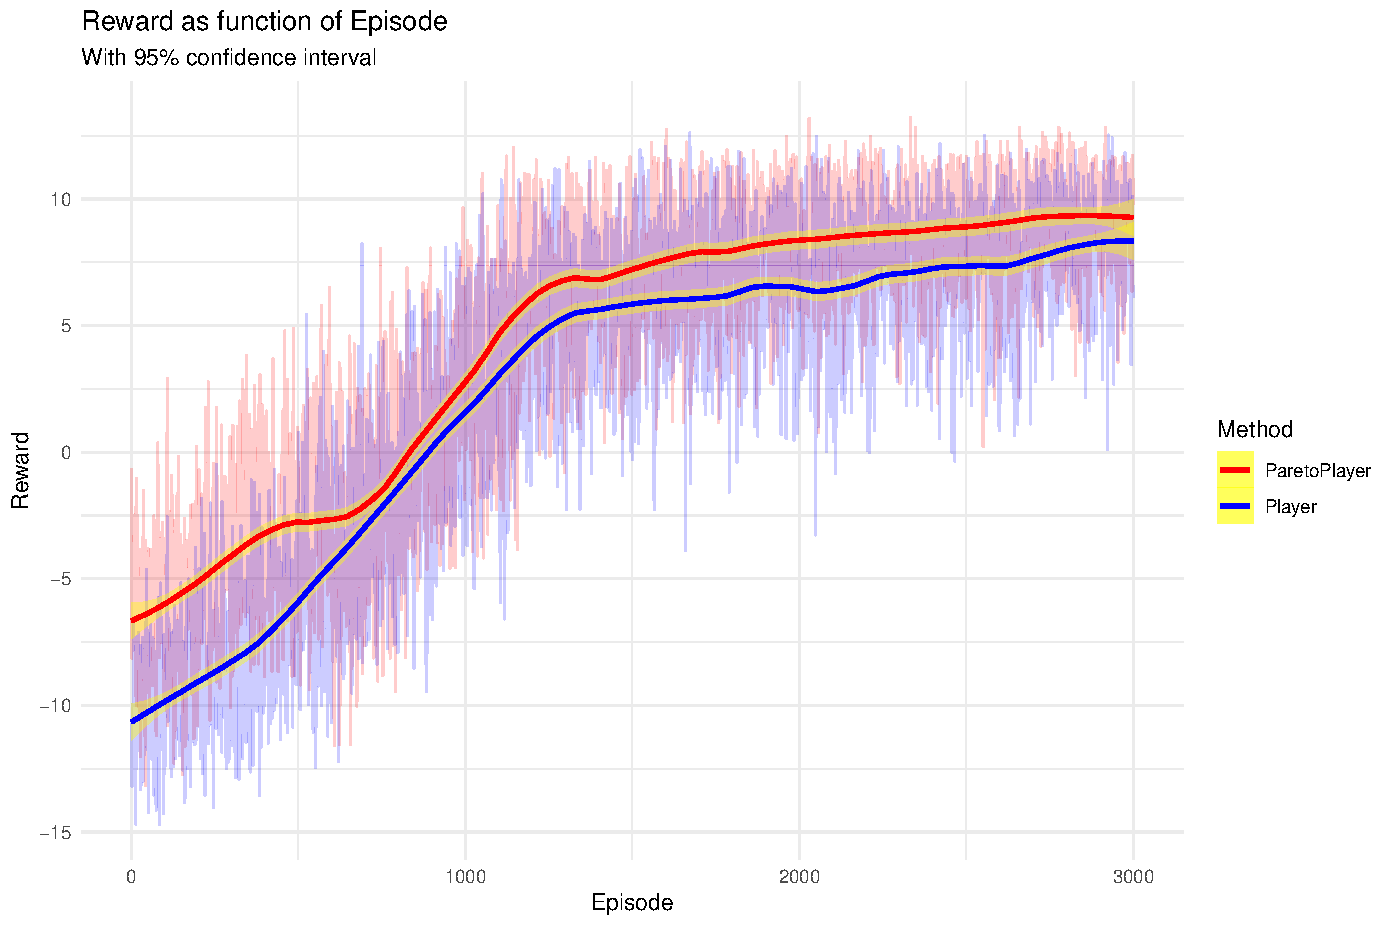
\includegraphics[width=0.8\linewidth]{images/reward_on_episode.pdf}
    \caption{Row-mean reward per episode for Pareto and ParetoPlayer}
    \label{fig:reward_per_episode}
\end{figure}

\begin{figure}[H]
    \centering
    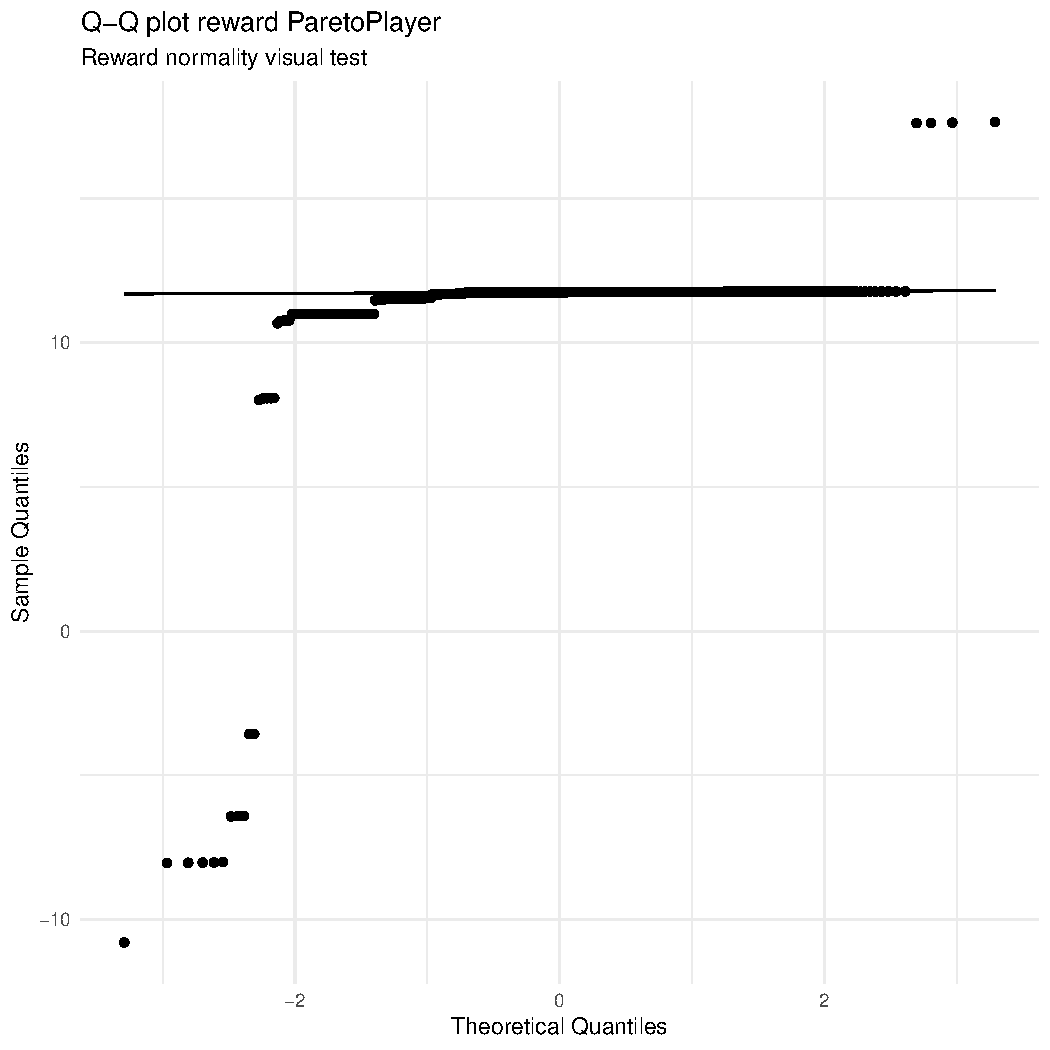
\includegraphics[width=0.6\linewidth]{images/Normality_QQ_Pareto.pdf}
    \caption{Quantile-Quantile plot episode reward computed on $1000$ battles during ParetoPlayer model evaluation}
    \label{fig:qq_pareto}
\end{figure}
\begin{figure}[H]
    \centering
    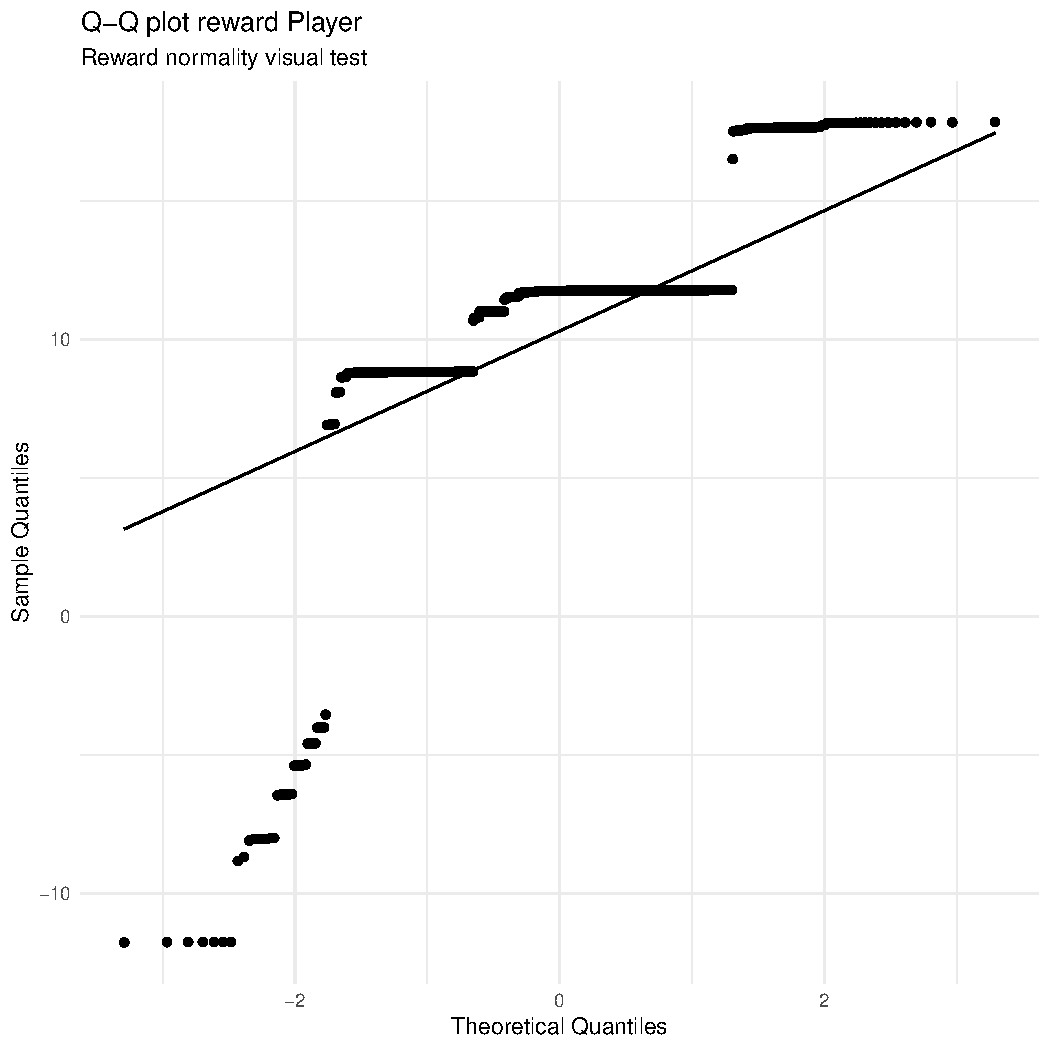
\includegraphics[width=0.6\linewidth]{images/Normality_QQ_Random.pdf}
    \caption{Quantile-Quantile plot episode reward computed on $1000$ battles during Player model evaluation}
    \label{fig:qq_random}
\end{figure}

\begin{figure}[H]
    \centering
    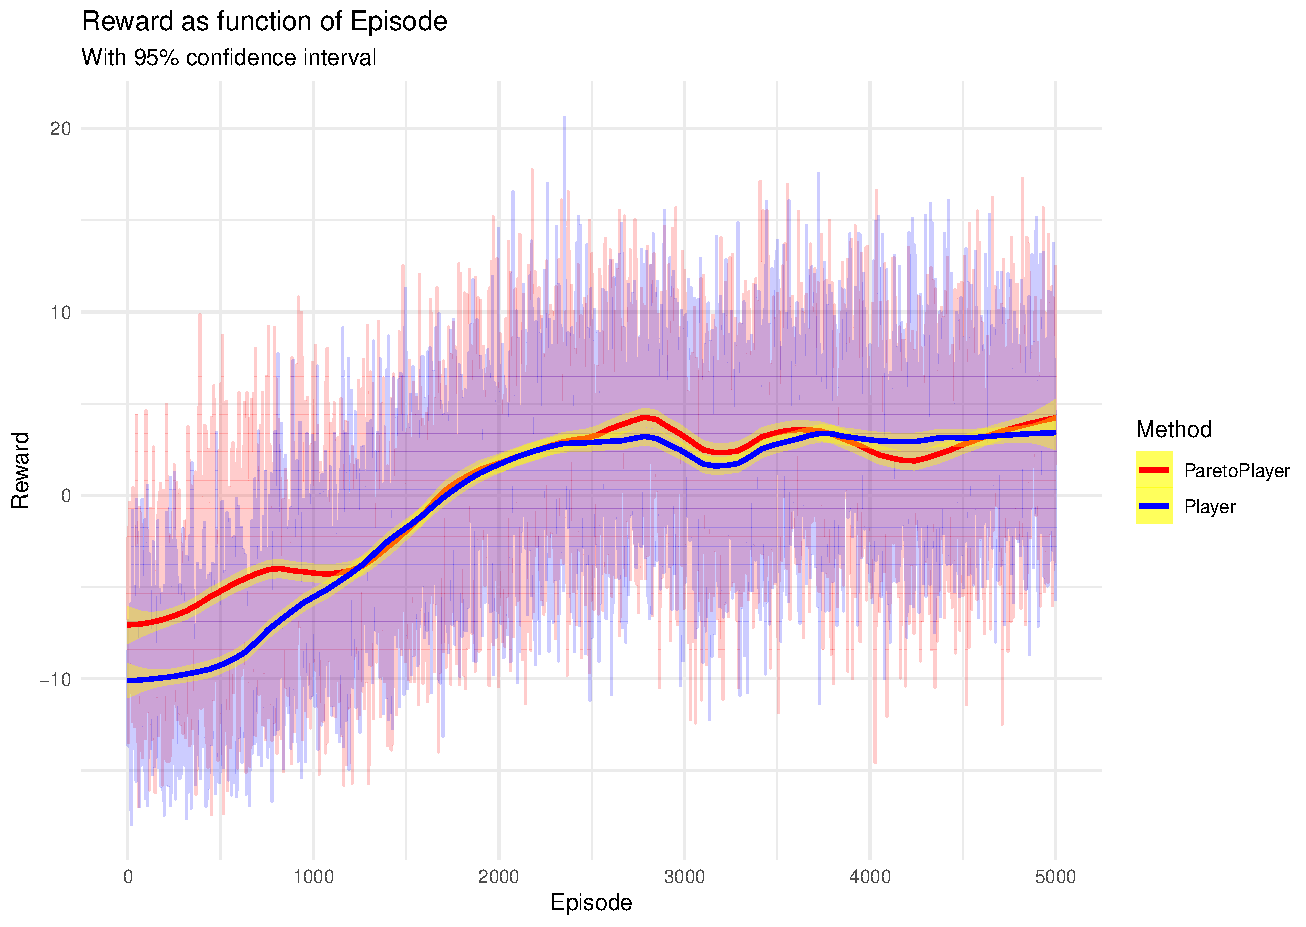
\includegraphics[width=0.8\linewidth]{images/rewardasfunctionofepisode2.pdf}
    \caption{Row-mean reward per episode for Pareto and ParetoPlayer (with variable enemy team)}
    \label{fig:reward_per_episode_var_team}
\end{figure}

\begin{figure}[H]
    \centering
    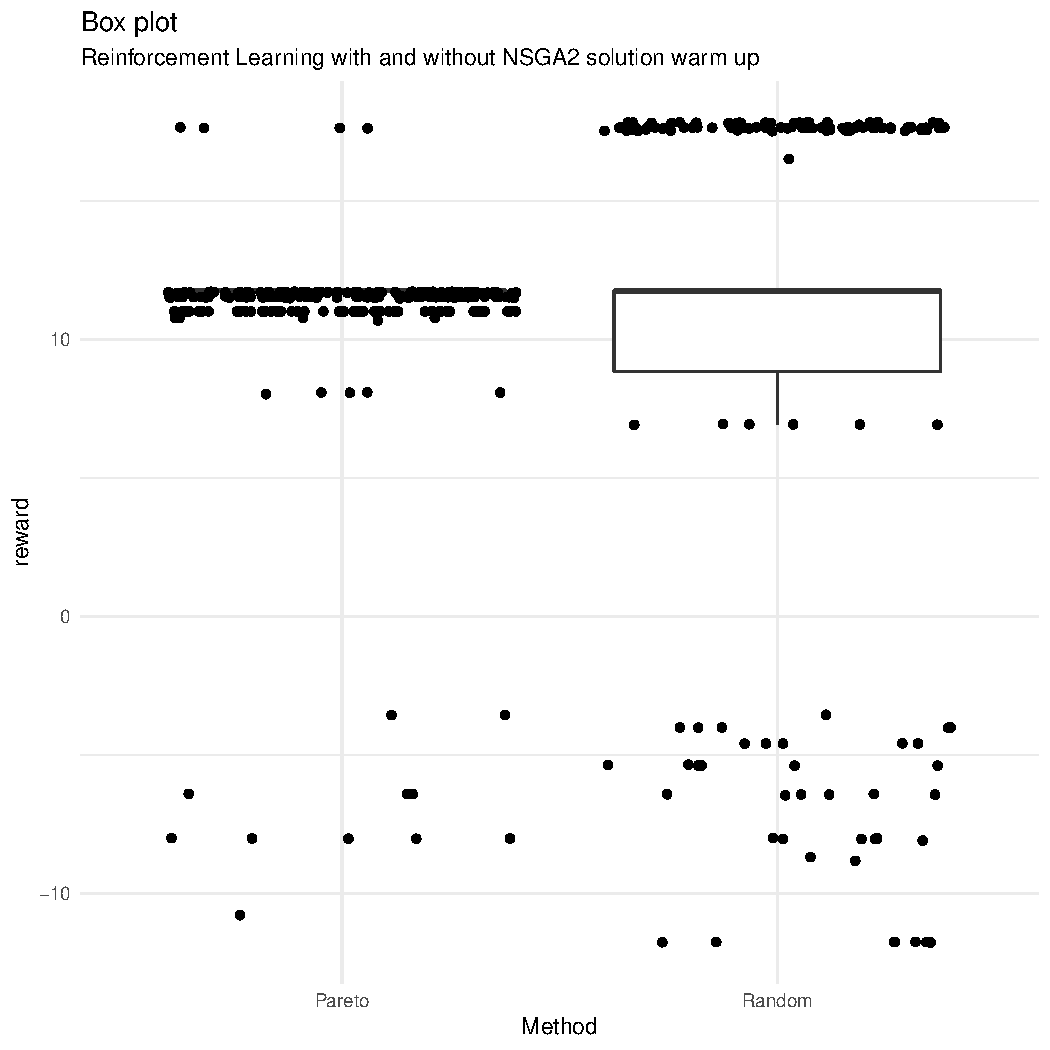
\includegraphics[width=0.6\linewidth]{images/box_plot_2v2.pdf}
    \caption{Box plot computed on $1000$ battles during ParetoPlayer and Player model evaluation}
    \label{fig:box_plot_2v2}
\end{figure}

\begin{figure}[H]
    \centering
    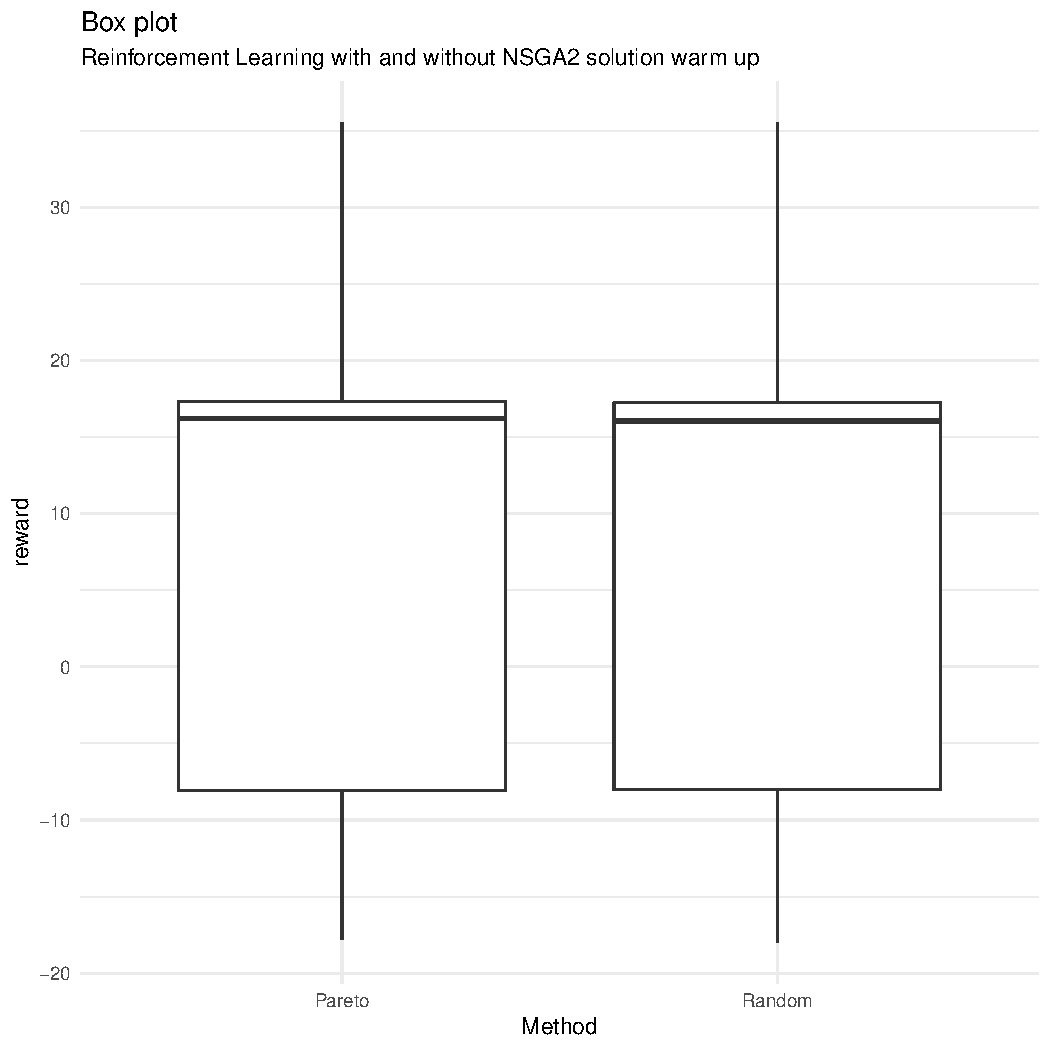
\includegraphics[width=0.6\linewidth]{images/box_plot_2v2_sampled.pdf}
    \caption{Box plot computed on $1000$ battles during ParetoPlayer and Player model evaluation (with variable enemy team)}
    \label{fig:box_plot_2v2_sampled}
\end{figure}

\end{document}